\documentclass[twoside,leqno,twocolumn]{article}
\usepackage{ltexpprt}

% -- Grace inserted --
\usepackage{amssymb}
\usepackage{graphicx}
\usepackage{subfigure}
\usepackage{amsmath}
\usepackage{multirow}
\usepackage{mathrsfs}
\usepackage{algorithm}
\usepackage[noend]{algorithmic}
\usepackage[usenames,dvipsnames]{color}
\usepackage{tabularx,booktabs}
\usepackage{bm}
\usepackage{cite}
% -- Grace inserted end --

\begin{document}

\title{\Large Real-time Estimation of the Urban Air Quality with Mobile Sensor System}
\author{Anonymous Author(s)\\
Affiliation\\
Address\\
email}

\maketitle

\begin{abstract} \small\baselineskip=9pt
Recently, real-time air quality estimation has attracted more and more attention from all over the world, which is also useful to our daily life. With the prevalence of mobile sensor, there is an increasingly available way to monitor the air quality with mobile sensors on vehicles, different from traditional expensive monitor station. In this paper, taking advantage of air quality data from mobile sensors, we propose an real-time urban air quality estimation method based on the Gaussian Process Regression for air pollution of the unmonitored areas. In our model, we present a kernel function to measure the distance among the spatio-temporal, climate and pollution features. In order to meet the real-time demands, we propose a two-layer ensemble learning framework and apply KD-Tree to improve adaptivity and computational efficiency. We evaluate our model with real data from mobile sensor system of Beijing, China, and the experiments show that our proposed model is superior to the state-of-art spatial regression methods in both precision and time performances.
\end{abstract}

\section{Introduction}
\noindent In recent years, air quality has attracted increasingly attention from all over the world. High levels of surface-level air pollutions are responsible for a range of disease. Nowadays, air quality monitor stations have been built to inform people about air quality every hour in many cities. However, it is so expensive to establish and maintain air quality monitor stations which only provide sparse information about the spatial distribution of air pollutants. Due to the sparsity of observation from static stations, many existing methods are good at coarse-grained estimation not fine-grained on time, usually a week, a month or even a year\cite{Hsieh2015Inferring} \cite{Grover2015A}. However, compared to coarse-grained estimation, real-time estimation is more significant to people's daily life to some extent\cite{Zhang2012Real}.
\begin{figure}[tbp]
\centerline{
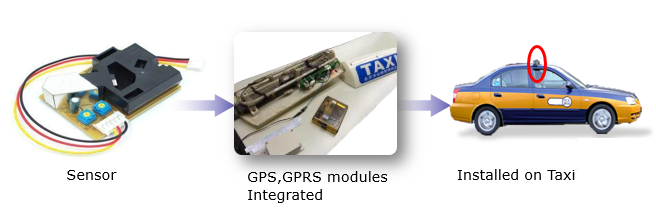
\includegraphics[width=1.0\linewidth]{pictures/equipment.png}
}
\caption{\label{fig:equipment}A mobile sensor for monitoring air quality located on the taxi}
\end{figure}

With the prevalence of mobile sensor which is available and affordable compared with traditional monitor station, there is an emerging way to monitor the air quality by the mobile sensor, which can provide abundant and fine-grained monitoring data. In this paper, the experiment dataset is from mobile sensor system of Beijing, China which consists of 51 taxis equipped with mobile sensor to monitor the concentration of $PM_{2.5}$ (Fig.\ref{fig:equipment}). The monitoring frequency is once every 30 seconds, which leads to the generation of about 35 thousands monitoring data every day. Especially the spatio-temporal distribution of monitoring positions is random depending on where the taxi wants to go, which can be seen in Fig.\ref{}. The abundant dataset gives us an opportunity to do real-time air quality estimation.

There are some challenges to do real-time estimation with monitoring data from mobile sensors. The one is the contradiction between the huge amount of data and the high demand time performance of real-time application. The second challenge is how to improve the adaptivity of real-time estimation model. The third challenge can be seen in \ref{}, which is the spatio-temporal distribution of monitoring data is non-uniform. If we just use latest observation to do the real-time estimation, it's difficult to get reliable results on these areas with sparse observations. So how to make full use of historical information and diffusion of air pollutant is a challenge.

To improve the time performance, we apply enhanced KD-tree to organize the original data into multiple homogeneous data sets and train an individual learner for each homogeneous data set. And then the estimations from these individual learners can be integrated based on ensemble learning. In order to enhance the adaptability of model, we propose a two-layer framework based on time slices. Besides, the pollution of a region depends on its own land use and dispersion from other places. To solve the problem of non-uniform spatio-temporal distribution of data, a new data sampling mechanism is proposed to select more related data for the query point, which combines the principle of pollutants generation.

The main contribution of this paper can be summarized as follows:
\begin{enumerate}
 \item We present a Real-time Ensemble Estimation Model (REEM) based on Gaussian Process Regression, which takes advantage of air quality observations from mobile sensors located on the taxis,
 \item We introduce a kernel function to discovery the pattern of the spatio-temporal, climate and pollutions features,
 \item We propose a selection mechanism to obtain more related observations for a given query point,
 \item We present a two-layer framework ensemble learning model based on time slice and apply KD-tree to improve adaptivity and computational efficiency,
 \item Experiments show that our proposed method outperforms the traditional spatial regression method in both precision and time cost.
\end{enumerate}
The rest of the paper is organized as follows: We next conclude related work. In section of preliminaries, we define our problems and review the Gaussian Process Regression. We describe the technical details of our approach in section 4. In section 5, the results of experiments on real-world data can be found, and we also evaluate it against state-of-art approaches. Finally, we conclude with a brief summary and discuss future work in section 6.

\section{Related Work}
In general, there are two kinds of main techniques for real-time air quality estimation \cite{Waylang}:

Deterministic model, which follows the principle of atmosphere dynamics, simulate the transport and diffusion of atmospheric particulate matter with a series of physical and chemical equations. Usually, these model are sophisticated and good at coarse-grained estimation. \cite{zhang2008online}\cite{Pfender2006Use}

Statistical approaches: Existing real-time estimation models based on measurements are either too simple to lead to low accuracy, such as the Inverse Distance Weighted(IDW), where the distance between query point and sample points is weighted average, or high computational complexity which cannot adapt the demand of real time, e.g. Kriging \cite{odeh1995further} or standard Gaussian Process Regression(GPR) \cite{rasmussen2006gaussian}, whose computation complexity is $O(N^3)$ with a set of N training set. In recent years, there have been some state-of-art model, which found the balance between accuracy and computational complexity. \cite{guizilini2015nonparametric} introduce a method, a Nonparametric Online Model(NOM), for the continuous online prediction of particulate matter in the air given sparse sensor information, which apply sub-sampling based on frequency analysis to reduce the computational complexity.  \cite{Nguyen2008Local} propose Local Gaussian Process Regression(LGP) for real-time estimation. But these methods are based on sparse data sets, usually from air quality monitor stations.

The method of collecting data by mobile sensor has attained much more attention recently due to its low cost, portability and easy maintainance \cite{Hasenfratz2015Deriving}. The mobile sensor for air quality monitoring was originally installed on public transportation which has a relatively fixed route\cite{Devarakonda2013Real}\cite{Jutzeler2014A}. And then, more and more private cars are installed with mobile sensors, which can collect a broader area of data. As the sensors become smaller, there is a trend that handhold  mobile devices become a method for data collection.

Because of a large amount of data from mobile sensors, it is a challenge to use mobile data for real-time application.
(However, there is no available real-time application when using a large amount of data from mobile sensors.)

\section{Preliminaries}
Air quality estimation is essentially a regression problem. For a set of N air quality observations $T=\{\bm{X_i}, y_i\}^N_{i=1}$ with $\bm{x_i}=(x_i^{spatio}, x_i^{time}, x_i^{weather})$ containing space, time and weather components and $y_i$ which is the concentration of pollutants at query points, our goal is to learn a transformation function $f(\bm{x_i})$ mapping the inputs $\bm{x_i}$ into the pollutant value given $y_i = f(\bm{x_i})+\varepsilon$, where the $\varepsilon$ usually represents noisy.

Gaussian Process extend multivariate Gaussian distribution to infinite dimensionality, which is determined by the mean function $m(\bm{x})$ and the kernel function $k(\bm{x},\bm{x}')$, Usually, we set the mean function $m(x)$ as zero function . We note:
\begin{equation}
 f(\bm{x}) \sim GP(0, k(\bm{x}, \bm{x}'))
\end{equation}
the joint distribution of observed values and predicted value for a query point $x_*$ is given by:
\begin{equation}
    \left[ {\begin{matrix}
	  	y\\
	  	y_*
	 \end{matrix}} \right]
   \sim
   {\rm N}(0,\left[ {\begin{matrix}
	  {K(X,X) + \sigma _n^2{I_n}}&{K(X,{x_*})}\\
	  {K({x_*},X)}&{K({x_*},{x_*})}
	 \end{matrix}} \right])
\end{equation}
Following the Bayesian paradigm, we can get the posterior probability distribution of $y_*$:
\begin{equation}
 y_*|x_*,X,y \sim N(\bar{f}(x_*), \mathbb{V}[f(x_*)])
\end{equation}
Where,
\begin{equation}
\begin{aligned}
 \bar{f}(x_*)&=K(x_*, X)[K(X,X)+\sigma_n^2\bm{I}]y \\
 \mathbb{V}[f(x_*)]&=K(x_*, x_*)-K(x_*, X)(K(X,X)+\sigma_n^2\bm{I})^{-1}K(x_*, X)
\end{aligned}
\end{equation}
We can get best estimation $y_*=\bar{f}(x_*)$.

The hyper-parameters of Gaussian process are $\theta=[\theta_k, \sigma_n]$, where the $\theta_k$ is the kernel function parameter and the $\sigma_n$ is the noise parameters. We can get the optimal value for a certain data set by maximizing the log marginal likelihood(Equation\ref{equ:likehood}) using common optimization algorithms.
\begin{equation}
\label{equ:likehood}
\bm{p}(y|X,\theta)=-\frac{1}{2}y^TK^{-1}y-\frac{1}{2}log|K|-\frac{n}{2}log2\pi
\end{equation}

Thus it can be seen that the main limitation of GPR is that the computational complexity is $O(n^3)$ with the training examples n. Especially, GPR is not appropriate for real-time estimation when training large amounts of data.

%--- luke

\section{Real Time Ensemble Estimation Model}

As discussed before, the data sampling frequency of mobile sensor is high for about 2 times per minute. To make full use of the dataset, we apply the whole data set as a training set instead of a data subset. However, the standard GPR is time-consuming, which makes it hard to adjust hyper-parameters immediately based on up-to-date data.

Based on ensemble learning method, we divide the data based on KD-Tree and train several individual learners of GPR. During prediction processes, we assemble the result of each individual learner.  Besides, we propose an adjustment framework of two-layer model based on time slice to suit the real-time environment, and apply the KD-tree to improve the efficiency.



%%Notation
%\begin{table}[!ht]
%\footnotesize
%\caption{Notation}
%\label{tab1}
%\def\tabblank{\hspace*{10mm}}
%\renewcommand{\multirowsetup}{\centering}
%\begin{tabularx}{0.5\textwidth}
%{@{\tabblank}@{\extracolsep{\fill}}cccp{100mm}@{\tabblank}}
%\toprule
 % Variable & Discription\\\hline
  %$N$ & size of training set \\
  %$\bm{y}=\{y_i\}^{N}_{i=1}$ & Observations of air quality\\
  %$X= \{ \bm{x_i} \}^{N}_{i=1}$ & Features of air quality\\
  %Spatio-Temporal Coordinates\\
  %\multirow{2}{*}{  $\bm{x_i}=\{x, y, t,\bm{\omega}\}_i$ } & Latitude, Longitude, Time \\
%& and Weather Features\\
%$d_{tree}$ & Depth of KD-Tree\\
%$\kappa$ & \\

%\bottomrule
%\end{tabularx}
%\end{table}

\subsection{Ensemble Estimation based on KD-Tree}

In common spatial interpolation problem, there is a basic assumption that the output should be similar if two samples are close to each other in spatial. Besides, many researches of estimation have also considered the temporal periodicity of pollutant[AAAI 15]. But we can see that it's more difficult to learn both the adjacency simularity and periodicity than just learn the former one. According to Occam's razor, given several models of similar performance in sufficient training set, the generalization ability of simplier model is better. Most state-of-the-art researches are based on base station data and less of sufficient training data in a short time. Once applied in large time span dataset, the temporal periodicity of data is improved and becomes hard to ignore. But in our circumstances, the data sampling frequency of mobile sensor is high that can aquire plenty data in a short time. The data has the characteristics of strong spatio-tempory adjacency simularity and weak periodicity. Thus we consider more of adjacency simularity rather than temporal periodicity in data partition and prior knowledge.

In ensemble learning field, the result of prediction or classification is better when each individual learner contains as much homogeneous data as possible.
Therefore we use temporal and spatial features to divide data based on KD-tree, so as to make the best homogeneity of each data subset and improve the computational efficiency.
%But considering the special property of moble sensor data in our circumstances(i.e. plenty of data is collected in a short period of time), the training data has the characteristics of strong spatio-tempory adjacency simularity and weak periodicity.

\subsubsection{Partition and Training of Individual Models based on KD-Tree}

Based on the discussion above, we use the spatio-temporal distance of samples to be the measure of division. To reduce the time cost of training and self-adapting of model, we use KD-tree to maintain the whole training set and divide the data efficiently based on the feature of balanced binary tree of KD-tree. We set the threshold as $\kappa\in[1,d_{tree})$, where $d_{tree}$ is depth of the KD-Tree, and select the $d_{tree}-\kappa$'th layer as dividing layer. The subtree this layer's nodes and ancestor nodes form each training subset.

As shown in the picture \ref{fig:KD-Tree}, each node represent a dividing sample and the number represent node id. The $\kappa$ is set to be 3. Now it is divided into 2 subset:
\[
\begin{split}
	&S_1 = \{\bm{x_0},\bm{x_1},\bm{x_3},\bm{x_4},\bm{x_7},\bm{x_8},\bm{x_9}\} \\
	&S_2 = \{\bm{x_0},\bm{ x_2}, \bm{x_5}, \bm{x_6}, \bm{x_{10}}, \bm{x_{11}}, \bm{x_{12}}\}.\\
\end{split}
\]

%insert picture(eps) (using command "convert name.png name.eps")
\begin{figure}[htbp]
\small
\centering{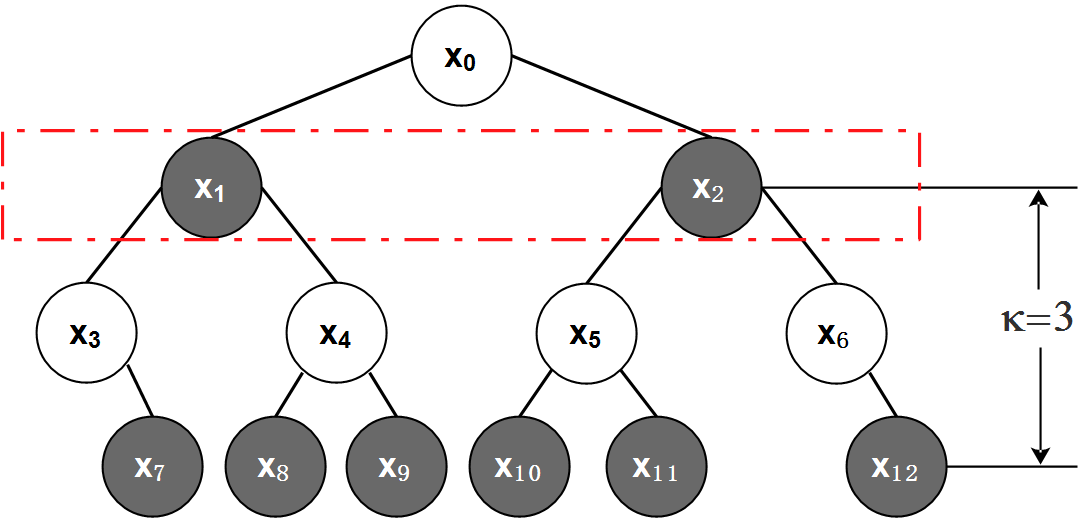
\includegraphics[width=0.5\textwidth] {pictures/KD-Tree4.png} }

\caption{A Sample of KD-Tree Structure}
\label{fig:KD-Tree}
\end{figure}
As KD-tree is balanced binary tree, the number and scale of data subset can be decided to make sure that the size of datasets is basically the same. That is:
\[
	m=2^{d_{tree} - \kappa}
\]
\[
		\forall i\in[1,m],\quad  d_{tree} - \kappa + 2^{\kappa-2}<|S_i| < d_{tree} - \kappa + 2^{\kappa}.
\]
where $m$ is the number of training subsets and $S_i$ is the $i$'th training subset.

Based on each training subset, we train more than one individual GP models. GPR allows to reflect the prior knowledge of the problem by designing kernel function. Based on the strong spatio-tempory adjacency simularity and weak periodicity. of data, our kernel is:
\begin{equation}
\begin{split}
	k_f(x,x') = &\sigma_{\omega}^{2}exp\{-\frac{1}{2}D^T_{wheather}MD_{weather}\}+\\
	&\sigma_{s}^{2}exp\{\frac{||D_{spatio}||^2}{l_s}\} + \sigma_{s}^{2}exp\{\frac{||D_{time}||^2}{l_t}\}\\
\end{split}	
\end{equation}
where $D_i = x_i - x'_i,  M=diag(\bm{l_w})$.

As can be seen that the value of kernel function reflects the spatial distance of samples after mapping, which is the covariance of samples. Considering the Gaussian noise in our observations, the final kernel function is:
\begin{equation}
\bm{K}(\bm{X},\bm{X})=\bm{K_f}(\bm{X},\bm{X'})+\sigma_n^2\bm{I}
\end{equation}
We define a GPR model under air quality estimation situation, which involves the following hyper-parameters:
\[
\bm{\theta}=(\sigma_s^2, \sigma_t^2, \sigma_\omega^2, l_s, l_t, l_\omega, \sigma_n^2).
\]

\subsubsection{Data Filtering Mechanism}
The Fig.x\ref{} illustrates the spatio-temporal distribution of mobile monitoring data is non-uniformed. So it is hard to obtain reliable estimations with latest monitoring data especially on these areas with sparse observations. This can be solved to train model with history monitoring data so that our model can use the discovered pattern to fit various distributions of observations. In order to reduce the computation complexity with amount of history monitoring data, we introduce a filtering mechanism to refine training data set for each query point.

As mentioned before, the similar data on space and weather feature can be organized into the same individual learners through the enhanced KD-tree. the reason why we don't choose the time feature as a standard to construct KD-tree is that the adjacent similarity of the data guaranteed by KD-tree can not characterize the periodicity of the time feature. So, we apply filtering mechanism to discovery the pattern of time feature and refine the training data of each individual learners. The filtering rule can be defined as follows:

\begin{align}
\{ X, y \}_{x_*}^a = \{ ~(x, y)_n ~&|~ k_t^a(x_*, x_n) > \delta \sum_{i=1}^N k_t^a(x_*, x_i) ~ \}_N \label{equ:filteringrule} \\
S_{x_*} =& \{ X, y\}_{x_*} = \bigcup_{a=1}^A\{x, y\}_{x_*}^a \notag
\end{align}
where
\begin{equation}
\begin{split}
k_{t}(x_*, &x) = \sum_{a=1}^A k_t^a(x_*, x) \\
&=\sum_{a=1}^A w_a^2 exp\{-2 \pi^2 r^2 \sigma_a^2\}cos(2\pi r \mu_a) \label{equ:k_t}
\end{split}
\end{equation}
Here, formula \ref{equ:k_t} is kernel function of time $r = x_*^{time}-x^{time}$ which can reflect the correlation of two points. As a multiplier of our model kernel function $k(x_*, x)$ (formula \ref{}), if $k_t(x_*, x)$ is micro, $k_(x_*, x)$ is also small, which means the correlation of the two points is weak. So, we can use a threshold and remove all data which fall below this threshold. Especially $\delta$ is a constant and N is the number of training data in a certain individual learner. $\{X, y\}_{x_*}^a$ (Formula \ref{equ:filteringrule}) means a most correlated data set in a certain frequency $\bm{a}$ for the query point $x_*$. And $S_{x_*}$ is called the estimation set for the query point $x_*$.


\subsubsection{Ensembling and Prediction}
The extent of pollution in a region is determined by the cumulative effect and the propagation effect. The cumulative effect of pollutants is related to the land use of a region and have its own regularity and periodicity in terms of time. While the propagation effect corresponds to the spread of pollutants and is weather-driven and distance-driven, that is, with obvious adjacent similarity.

The estimation model based on enhanced KD-tree ensures the adjacent similarity of the data sets corresponding to each individual learner in the weather and spatial features. So for a given query point $x_*$, the nearest individual learner $L_{nearest}$ can be found with enhanced KD-tree, data filtering mechanism should be applied to the data set of $L_{nearest}$ to refine a most correlated data as estimation data set, which reflect the cumulative effect of pollutant in the query point. To other individual learners of our model, we choose the latest monitoring data as their estimation data set, which reflect the propagation of pollutants. Finally, the estimation for a value $y_*$ is performed using weighted averaging over $m$ individual predictions $y_*^{(i)}$. After formal definition, we can train each subset based on the GPR method as discussed above:
\begin{equation}
y_*=\frac{\sum_{i=1}^mw_iy^{(i)}_*}{\sum_{i=1}^mw_i}
\end{equation}
we use the kernel average of $x_*$ directly in each estimation data set to be the weight of ensembling, to further improve the computation efficiency of prediction and train.
 \begin{equation}
 w_i =  mean(\bm{K}(*,\bm{X^{(i)}}))
 \end{equation}
The detail can be seen in Algorithm \ref{}.
\begin{algorithm}[htb]
\caption{Ensembling Prediction}
\begin{algorithmic}[1]
\REQUIRE ~~\\
the query point $x_*$
S
\STATE $S_{estimation}$
\STATE $S_{nearest} = FindNearestLearner(S_{estimation}, x_*)$
\STATE $S_{nearest}^* = DataFilteringMachanism(S_{nearest})$
\STATE $y_*^{nearest} = GP(S^{nearest}_*)4 $
\FOR{$ \bm{S_i} \in \bm{S-S_{nearest}}$}
    \STATE $S_i^* = FindLatestData(S_i)$
    \STATE $y_*^{(i)} = GP(S_i^*)$
\ENDFOR
\STATE $y_*=\frac{\sum_{i=1}^mmean(\bm{K}(*,\bm{X^{(i)}}))_iy^{(i)}_*}{\sum_{i=1}^mmean(\bm{K}(*,\bm{X^{(i)}}))}$
\STATE Output($y_*$)
\end{algorithmic}
\end{algorithm}

\subsection{Self-Adaption Framework of Two-Layer Model based on Time Slice}
To improve the adaptivity of model in real-time environment, we need to update the model according to the up-to-date data in time. The standard GPR uses new data to update the covariance matrix by calculating the inverse of matrix again, whose time complexity is O($n^3$) and can hardly match the real-time request. Besides, to adjust to the change of environment(e.g climate change, periodical change of time), the hyper-parameters need to be trained again when time span is large. However, the training of classical GPR is time-consuming, which makes it hard to adjust hyper-parameters immediately based on up to date data. In this paper, based on the high efficiency of KD-Tree insertion and deletion, we design a kind of two-layer updating framework, which applies different strategies to update the model in different lengths of time windows.

The figure \ref{fig:AF} is a diagram of self-adaption framework. Each small rectangle represents the data of one time slice. $T_l$ and $T_s$ are the thresholds we set, denoting the lengths of two time windows respectively. In the framework, the data in $T_l$ time window is used for training hyper-parameters and construction of KD-Tree, i.e.
\[
	\{\bm{X}, \bm{y}\}_{training}^h = \{(\bm{x}, y)~|~ x^{time} \in [h, h + T_l] \}
\]
where $h$ is current time slice.

%insert picture(eps) (using command "convert name.png name.eps")
\begin{figure}[htbp]
\small
\centering{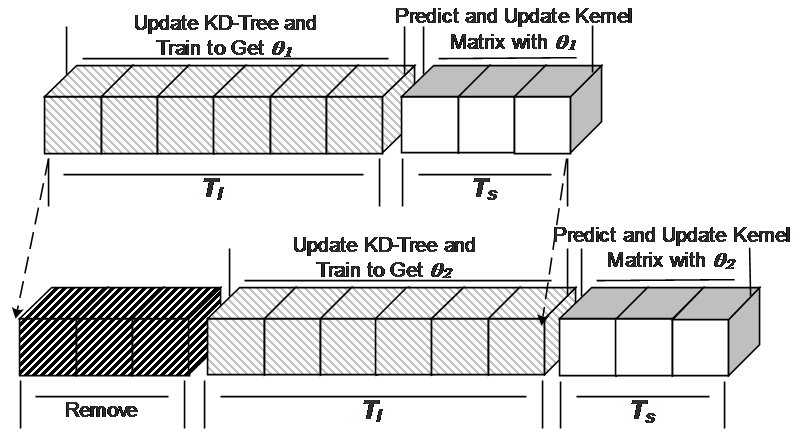
\includegraphics[width=0.5\textwidth] {pictures/Framework.png} }

\caption{Self-Adaption Framework}
\label{fig:AF}
\end{figure}

In our framework, we do not adjust hyper-parameters in every time slice because the length of a time slice is only 30 seconds and training for each time leads to a high time cost. Moreover, in a relative short period of time, due to the tempory adjacency simularity of data, the hyper-parameters will be changed little. So we use the same hyper-parameters for estimation and adjust the model adaptively through updating the training subsets as well as recalculating kernel matrices in the $T_s$ length of time slice after each training, i.e. for  a  new  sample $[\bm{x_{new}}, y_{new}]$��
\begin{equation}
	\begin{split}
	\bm{K^{(i)}_{new}} = &\bm{K}([\bm{X^{(i)}}, \bm{x_{new}}], [\bm{X^{(i)}}, \bm{x_{new}}]), \bf{if} ~ \bm{x_{new}} \in \bm{S^{(i)}}. \\
	\end{split}
\end{equation}

When the time reaches $T_s$ after training, we slide the training time window and remove stale samples $\bm{X_{remove}}$ from KD-Tree.
\[
	{\bm{X_{remove}}} = \{\bm{x}~|~ x^{time} \in [h - T_l - T_s, h - T_l]\}
\]
And the new samples $\bm{X_{add}}$ is added to KD-Tree.
\[
	{\bm{X_{add}}} = \{\bm{x}~|~ x^{time} \in [h - T_s, h]\}
\]
Due to the nature of KD-Tree, the efficiency of deletion and insertion is very high and the tree structure can be adjusted adaptively through the rotation of nodes to ensure the homogeneity of the data in each subset. And then each training subset will be trained again. The overall framework of the model is detailed in algorithm \ref{alg:MCT}.

\begin{algorithm}[htb]
\caption{Model Update and Prediction Framework}\label{alg:MCT}
\begin{algorithmic}[1]
\REQUIRE ~~\\
Initial training set, $\{\bm{X}, \bm{y}\}$\\
Threshold, $\kappa, T_l, T_s$
\STATE $//$ Build a new KD-Tree with $\bm{X}$
\STATE $Tree= Build(\bm{X})$
\STATE $//$ Data partition with KD-Tree and threshold $\kappa$
\STATE $\bm{S} = GetSubsets(Tree, \kappa)$
\STATE $//$ For every subset train a model
\FOR{$\bm{S^{(i)}} \in \bm{S}$}
   \STATE $\bm{K^{(i)}}=GPR(\bm{S^{(i)}})$
\ENDFOR

\STATE $\bm{S_{new}} = \varnothing$
\STATE $cnt=0$
\WHILE{$HaveNextTimeslice()$}
    \STATE $cnt$++
    \STATE $\{\bm{X_{new}}, \bm{y_{new}}\}=GetNewData()$
    \STATE $\bm{S_{new}} = \bm{S_{new}} + \{\bm{X_{new}}, \bm{y_{new}}\}$


     \IF {$cnt \mod T_s = 0 $}
        \STATE $\bm{Tree}$.DeleteBeforeTime($T_l$)
        \STATE $\bm{Tree}$.Add($\bm{S_{new}} $)
        \STATE $\bm{S} = GetSubsets(Tree, \kappa)$
        \FOR{$\bm{S^{(i)}} \in \bm{S}$}
              \STATE $\bm{K^{(i)}}=GPR(\bm{S^{(i)}})$
        \ENDFOR
         \STATE $cnt = 0$
         \STATE $S_{new} = \varnothing$
     \ELSE
        \FOR{$\{\bm{x_i}, y_i\} \in \{\bm{X_{new}}, \bm{y_{new}} \}$}
           \STATE $id = Tree$.find($\{\bm{x_i}, y_i\}$)
           \STATE $\bm{K^{(id)}} = \bm{K}([\bm{X}, \bm{x_{i}}], [\bm{X}, \bm{x_{i}}])$
            \STATE $\bm{y^{(id)}}=\bm{y^{(id)}} + y_i$
         \ENDFOR
      \ENDIF

    \STATE $//$ Predict with new Kernel
    \FOR {$\bm{x_*} \in \bm{S_w}$}
       \FOR{$i \in [1, m]$}
           \STATE $y_*^{(i)}=\bm{k_*^T}(\bm{K^{(i)}}+\sigma_n^2\bm{I})^{-1}\bm{y^{(i)}}$
       \ENDFOR
       \STATE $y_*=\frac{\sum_{i=1}^mmean(\bm{K}(*,\bm{X^{(i)}}))_iy^{(i)}_*}{\sum_{i=1}^mmean(\bm{K}(*,\bm{X^{(i)}}))}$
       \STATE Output(${\bm{x_*}, y_*}$)
    \ENDFOR
\ENDWHILE

\end{algorithmic}
\end{algorithm}

\subsection{Complexity Analysis}
In the training process, when using the maximum likelihood method, as the data set is divided into $m$training subsets, the time complexity of each iteration is O ($k^3$), where $k=\frac{n}m$. And for all subsets, the total complexity of the iteration O ($k^3\times m$).  The computational efficiency is greatly improved compared to the traditional GPR with O ($n^3$) time complexity. In addition, the time complexity of estimation is O($n$), so it can be applied to the real-time scenarios.

In the adaptive updating process of the model, the time complexity of KD-Tree insertion and deletion is O ($\log (n) $) which can be negligible. And the time complexity of recalculating kernel matrices is O ($k^3\times m$), which also has a greater improvement than the time complexity O($n^3$) of traditional GPR .

%--end luke --

\section{Experiments}
In this part, our model, Real-time Ensemble Estimation Model(\emph{REEM}), are evaluated using the climate data and the air quality data from mobile sensor system(Fig.\ref{fig:display}). The performance of \emph{REEM} is compared with the state-of-art interpolation models, e.g. standard \emph{GPR}, \emph{Kriging}, \emph{IDW}, \emph{NOM} and \emph{LGP}. Especially, the kernel function of standard \emph{GPR} is same with \emph{REEM}. The goal of models is to estimate the concentration of $PM_{2.5}$ at any given location.
\begin{figure}[!htb]
\centerline{
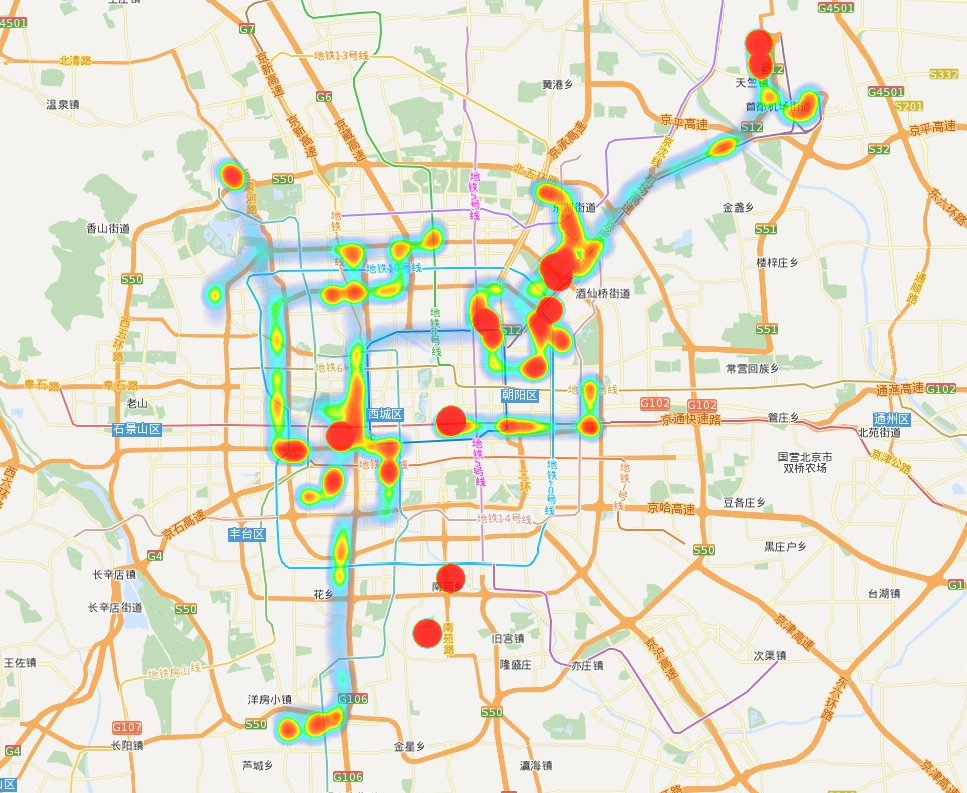
\includegraphics[width=0.68\linewidth]{pictures/display.png}
}
\caption{\label{fig:display}An real-time estimation result in Beijing at a certain time}
\end{figure}
\subsection{Data Set from Mobile Sensor System}
Our data set is from June 1st, 2015 to September 29th of totally 121 days, whose data sampling frequency is high for about 2 times per minute. The monitoring data is comprised of the sampling time, the concentration of $PM_{2.5}$, longitude and latitude. During this period, there are 51 mobile devices collecting data on road, while only several devices work at the same time. The number of records per day in June are shown in Fig\ref{fig:perday}, where the number is considerable and relatively stable. We also make an experiment to get the distribution of the number of records at every timestamp during one day. As shown in Fig\ref{fig:oneday}, the amount of records at different times fluctuates greatly, which is a challenge to real-time model.
\begin{figure}[!htb]
\centerline{
\subfigure{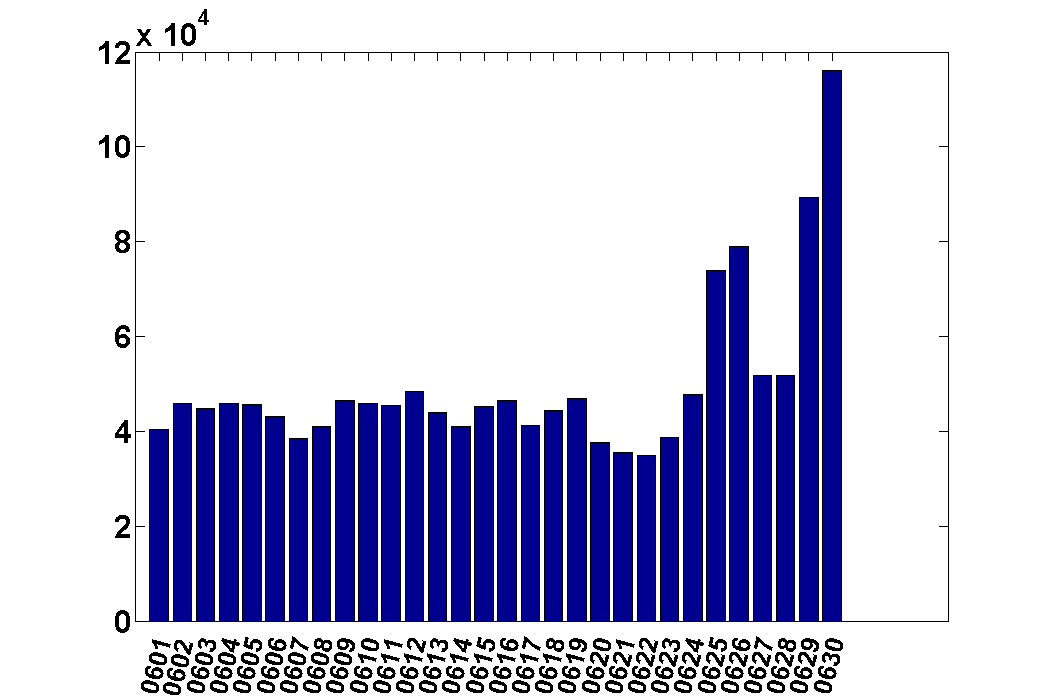
\includegraphics[width=0.48\linewidth]{pictures/recordsPerday.png}\label{fig:perday}}
\subfigure{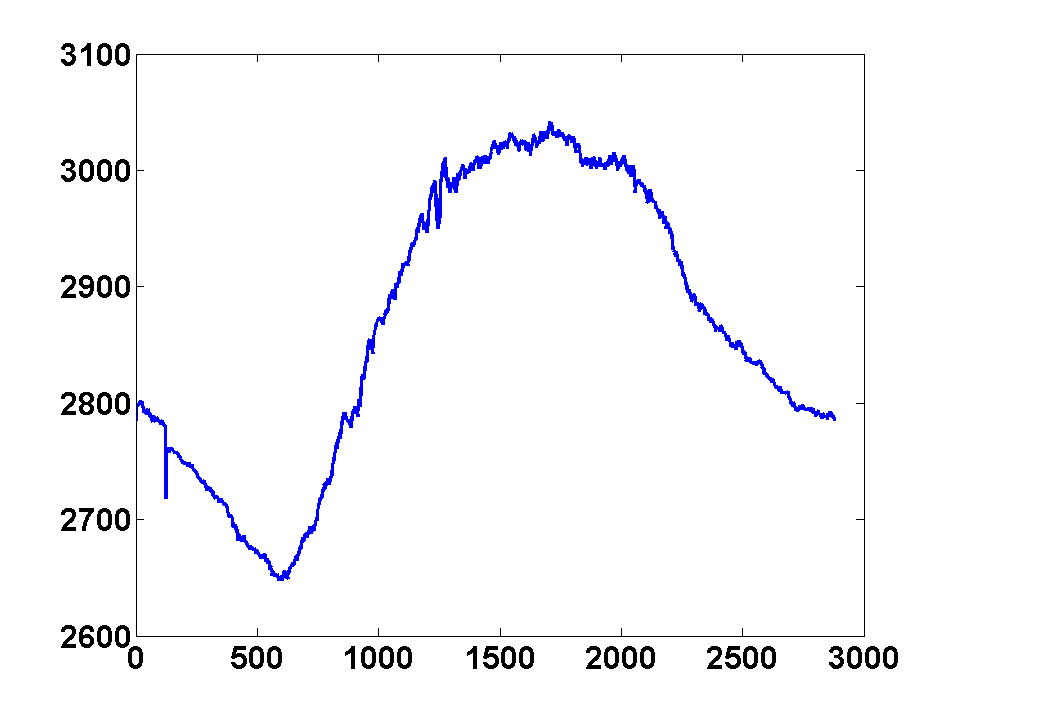
\includegraphics[width=0.48\linewidth]{pictures/recordsOneday.png}\label{fig:oneday}}
}
\caption{\label{fig:recordsPerday}Left:The number of records collected by mobile sensors per day in June. The horizontal coordinate x represents date, the format like '06XX' means XX days in June; the vertical coordinate y is the sampling volume; Right: The distribution of the number of records collected by mobile sensors at every timestamp during one day. The vertical coordinate y represents quantity of records; the horizontal coordinate x is timestamp, which of time interval is 30s}
\end{figure}


%\begin{figure}[!htb]
%\centerline{
%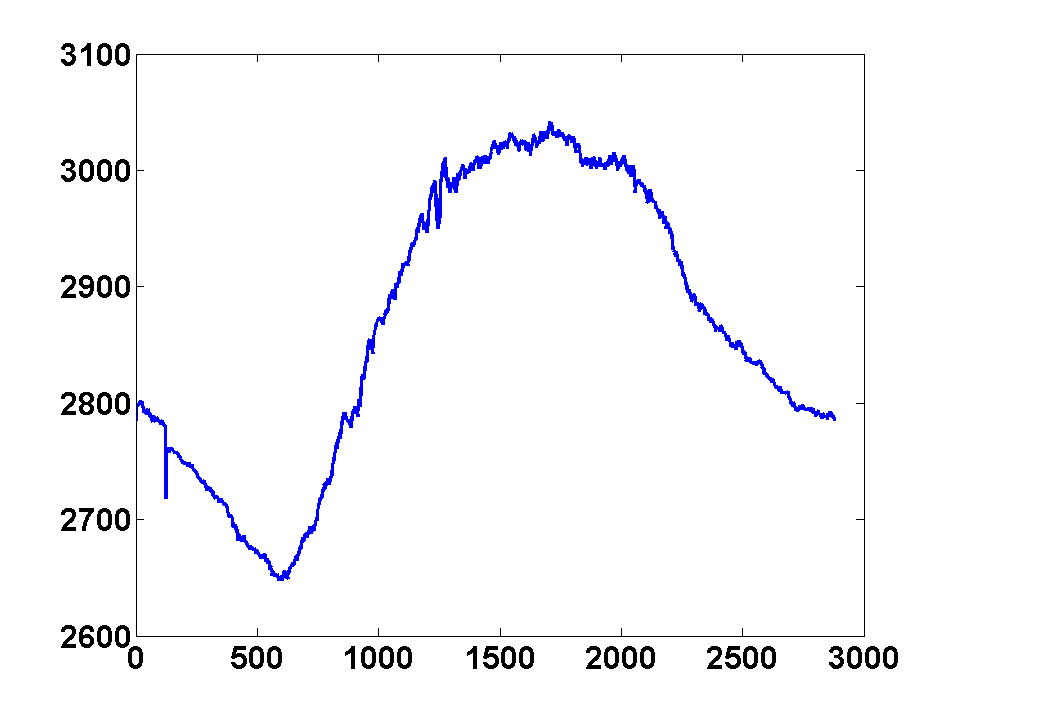
\includegraphics[width=0.72\linewidth]{pictures/recordsOneday.png}
%}
%\caption{\label{fig:recordsOneday}The distribution of the number of records collected by mobile sensors at every timestamp during one day. The vertical coordinate y represents quantity of records; the horizontal coordinate x is timestamp, which of time interval is 30s}
%\end{figure}

Based on the aforementioned analysis, in order to verify the validity and feasibility of models under different sampling densities, we take every one hour data as a segment and cluster these segments into several classes according to data volume. We validate models through 10-fold cross-validation.

\subsection{Kernel Selection}
The Mean Average Error(\emph{MAE}) of the evaluation on different variables combinations is presented in Table\ref{tab:kCombination}. The performance of spatial feature is good. Additionally, the great improvement generated by the incorporation of time feature, which is in line with our conclusion that mobile data has strong spatio-temporal adjacent similarity. As well as the improvement generated by the inclusion of all of them. So, the input features we choose for our model consist of time, longitude, latitude, temperature, rain, pressure, humidity.

\begin{table}[!ht]
\footnotesize
\caption{The comparison of evaluation on different variables combinations}
\label{tab:kCombination}
\def\tabblank{\hspace*{10mm}}
\renewcommand{\multirowsetup}{\centering}
\begin{tabularx}{0.5\textwidth}
{@{\tabblank}@{\extracolsep{\fill}}lccp{100mm}@{\tabblank}}
\toprule
  Feature & MAE \\\hline
  $K_{spatio}$ & 9.81 \\
  $K_{time}$ & 32.40 \\
  $K_{weather}$ & 19.52 \\
  $K_{weather}+K_{time}$ & 16.87 \\
  $K_{spatio}+K_{weather}$ & 10.67 \\
  $K_{spatio}+K_{time}$ & 8.87 \\
  $K_{spatio}+K_{time}+K_{weather}$ & 7.69 \\
\bottomrule
\end{tabularx}
\end{table}

\subsection{Accuracy Comparison}
Fig.\ref{fig:performance} shows the Logarithm Root Mean Square Error(\emph{LRMSE}) of evaluation on the test set for each size training set. As we can see from Fig.\ref{fig:performance}, the performance of \emph{LGP} is better than other models just when the training set is 100. This phenomenon is related with the strategy of LGP, which is a continuous online regression model and retrain model as long as a new observation is attained. The way of real time update alleviates the disadvantage of sparse information, while wastes the computing resource when data is enough. Besides, our model \emph{REEM}, which is based on ensembling local information, is superior to \emph{standard GPR}. This is follow the idea of ensemble learning which a set of weak learners based on local information can acquire more strong generalization ability. All in all, The estimation performance of our model is well. In most cases, the accuracy of our model outperforms other classic interpolation models, e.g. \emph{GPR}, \emph{Kriging} and \emph{IDW}, also is slightly better than online models, like \emph{LGP} and \emph{ONM}. Here, the \emph{LRMSE} is defined as:
\begin{equation}
LRMSE = log\sqrt{\frac{\sum_{k=1}^n(y_{estimation}-y_{ground})^2}{n}}
\label{equ:lrmse}
\end{equation}

\begin{figure}[!htb]
\centerline{
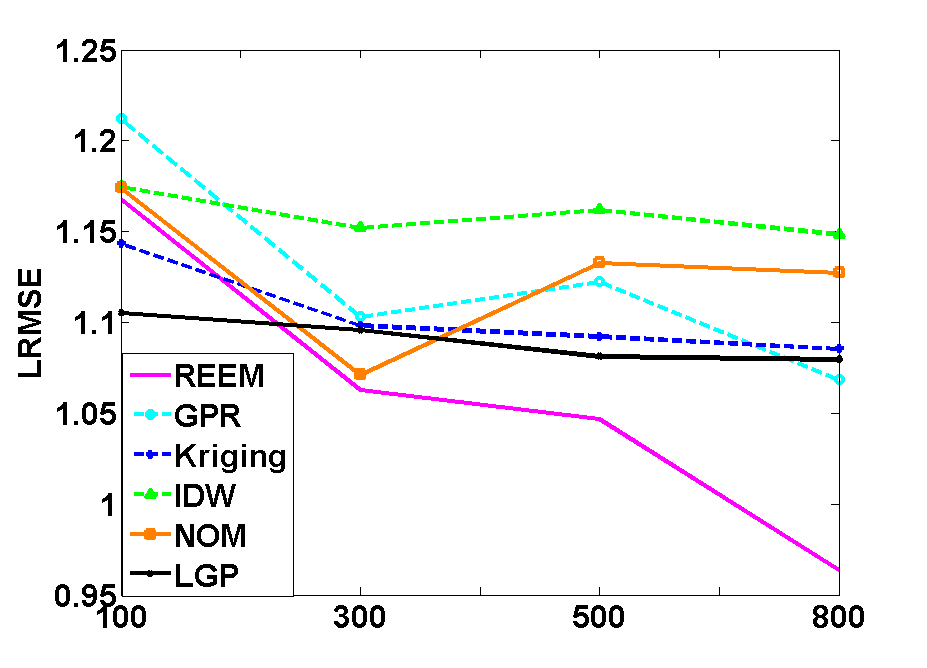
\includegraphics[width=0.72\linewidth]{pictures/performance.png}
}
\caption{\label{fig:performance}The LRMSE of evaluation on different training points(100, 300, 500, 800 data points, respectively)}
\end{figure}

\subsection{Time Cost Comparison}
As to real-time model, time cost, usually consisting of training cost and estimating cost, is a crucial criterion. Since LGP and IDW are online training model, Fig.\ref{fig:trainingtime} just illustrates the training time comparison among OEEM, GPR and Kriging, where we can see our model have obvious advantages. Besides, considering the average time in millisecond needed for estimation of 1 query point shown in Table\ref{tab:testingtime}, OEEM outperforms standard GPR, LGP and Kriging while being close to IDW.
\begin{figure}[!htb]
\centerline{
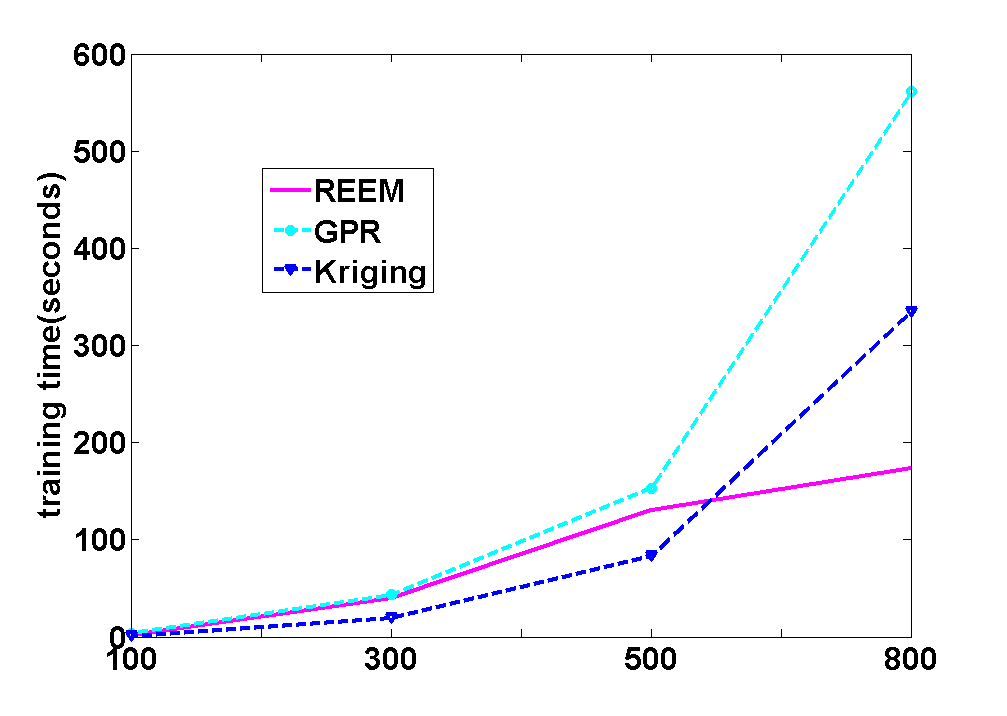
\includegraphics[width=0.72\linewidth]{pictures/trainingtime.png}
}
\caption{\label{fig:trainingtime}The comparison of training time on different datasets with decreasing training points}
\end{figure}

\begin{table}[!ht]
\footnotesize
\caption{The comparison of average time needed for estimation of 1 query location on different models}
\label{tab:testingtime}
\def\tabblank{\hspace*{10mm}}
\renewcommand{\multirowsetup}{\centering}
\begin{tabularx}{0.5\textwidth}
{@{\tabblank}@{\extracolsep{\fill}}lccp{100mm}@{\tabblank}}
\toprule
  model & querying time(millisecond) \\\hline
  REEM & 0.31 \\
  standard GPR & 0.73 \\
  LGP & 73.39 \\
  Kriging & 0.47 \\
  IDW & 0.22 \\
\bottomrule
\end{tabularx}
\end{table}

In conclusion, comprehensively considering the performance of accuracy and time, our model is the best-performing model.
\section{Conclusion and Future Work}
Our goal is to do real-time urban air quality estimation with mobile sensor system. We proposed and implemented Real-time Ensemble Estimation Model (REEM) based on GPR. We evaluated the model with mobile data from mobile sensor system. The Experiments showed our model outperforms other state-of-art models both on precision and time efficiency.

The next work we can do to improve the air quality estimation as follows:

The diffusion of pollutants in the air is sophisticated. There are many factors can influence the transportation. Inspired by the Land-Use Regression, we can integrate the city's POI information into our model. Besides, the spatio-temporal distribution of sampling positions is random depending on where the car with the sensor wants to go. So, we can design an algorithm for route planning in order to optimize the spatial distribution of observations. Actually, as to the air quality data from mobile cars, there is a problem need to be solved. Since the mobile sensor located on the car is close to pollution source, the monitoring data is higher than the truth. Based on supervising learning, We should try to design an algorithm to correct the observations from car with static monitoring station.

With the rapid development of mobile sensors, how to take full advantage of mobile data is a meaningful and challenging task.
% References and End of Paper

\bibliography{AQE_draft}
\bibliographystyle{sdm}
\end{document}
% end of Itexpprt.tex 